\documentclass[a5paper]{article}
\usepackage[a5paper, top=8mm, bottom=8mm, left=8mm, right=8mm]{geometry}

\usepackage{polyglossia}
\setdefaultlanguage[babelshorthands=true]{russian}

\usepackage{fontspec}
\setmainfont{FreeSerif}
\newfontfamily{\russianfonttt}[Scale=0.7]{DejaVuSansMono}

\usepackage[font=scriptsize]{caption}

\usepackage{amsmath}
\usepackage{amssymb,amsfonts,textcomp}
\usepackage{color}
\usepackage{array}
\usepackage{hhline}
\usepackage{cite}

\usepackage[hang,multiple]{footmisc}
\renewcommand{\footnotelayout}{\raggedright}

\PassOptionsToPackage{hyphens}{url}\usepackage[xetex,linktocpage=true,plainpages=false,pdfpagelabels=false]{hyperref}
\hypersetup{colorlinks=true, linkcolor=blue, citecolor=blue, filecolor=blue, urlcolor=blue, pdftitle=1, pdfauthor=, pdfsubject=, pdfkeywords=}

\usepackage{tabu}

\usepackage{graphicx}
\usepackage{indentfirst}
\usepackage{multirow}
\usepackage{subfig}
\usepackage{footnote}
\usepackage{minted}

\sloppy
\pagestyle{plain}

\title{Язык программирования Java, введение}
\author{Юрий Литвинов\\\small{yurii.litvinov@gmail.com}}

\date{??.09.2018}

\begin{document}

\maketitle
\thispagestyle{empty}

\section{Формальности}

Занятия будут раз в неделю. На занятиях я обычно буду что-то рассказывать (но немного, раз у вас есть хороший лекционный курс по Java), потом мы будем, собственно, практиковаться, решая прямо на паре несложные задачки с моей помощью. Однако основная практика будет в виде домашних заданий, которых будет много (поскольку единственный известный мне способ научиться программировать --- это много программировать, так же как нельзя научиться летать, читая книжки про самолёты). Кстати, я считаю, что учить собственно язык программирования нет особого смысла, потому что по Java полно хороших книг и читать все умеют, так что тратить время на парах на зачитывание вслух документации по языку и стандартной библиотеке мы не будем. Основной упор будет делаться (ну, насколько это возможно) на основные концепции, которые так или иначе выражаются в языке, типичные приёмы программирования, подходы и проблемы, так что при успешной сдаче этого курса вы сможете программировать не только на Java, но и на C\#, станете лучше программировать на C++, быть может, потратив пару дней на то, чтобы почитать, как те или иные штуки делаются на этих языках.

Для того, чтобы получить зачёт, надо будет сдать некоторый (большой!) процент домашних заданий, написать две контрольные. Сдавать решения надо будет, выкладывая их на гитхаб и делая пуллреквест. Если кто-то без идей, что это значит, я готов посвятить этому некоторое время на паре, потому что пользоваться гитом надо уметь и там реально есть что рассказать, а пока можно будет сдавать, присылая решения архивом. 

Куда присылая: есть система поддержки домашек, применяемая в СПбГУ, называется HwProj, её писали такие же второкурсники, как и вы, поэтому она может доставлять немного боли, зато вы сами можете поучаствовать в её разработке, если захотите. Адрес у неё \url{http://hwproj.me/}, там будут публиковаться условия задач, туда же надо сабмитить решения, там же будет обратная связь и табличка, где будут отмечаться сданные или несданные задачи. Там надо зарегаться и добавиться в курс с очевидным названием, подождать, пока я подтвержу регистрацию, и начать выкладывать туда домашки (в виде либо ссылки на пуллреквест, либо прямо архив с решением). Если там что-то не работает, непонятно, всё плохо, вы всё решили, но домашку съела собака, то есть зажевал HwProj, пишите мне на почту. Вообще, кстати, писать мне на почту --- хорошая практика, задавать любые вопросы можно, я буду стараться на них ответить. Стесняться не надо, в конце концов, помогать вам изучать предмет --- моя работа. Если потребуется более оперативная связь, есть джаббер, скайп, телеграм или google hangouts, но это можно запросить по почте. В качестве среды программирования можно использовать то, что вам больше нравится, но мы будем писать относительно большие программы, поэтому блокнот или vim не очень подойдут. Я рекомендую IDEA (потому что на мой вкус она самая удобная), но не настаиваю, к тому же, я предвзят, потому что сам имею некоторое отношение к JetBrains.

Ещё обратите внимание, что просто сделать домашку может быть недостаточно. Я, как практикующий программист, не хочу учить вас писать правильно работающие программы, мне интереснее специалисты, которые пишут сопровождаемые, расширяемые, документированные и т.д. программы, про различие программы и программного продукта вы, наверное, слышали (если нет, я расскажу как-нить). Поэтому большая часть мучений будет со стилем кодирования, хорошими практиками, разумностью архитектуры и подобными вещами, если программа выдаёт правильный ответ, это ни о чём не говорит. Строго говоря, критерии приёмки таковы: задача зачитывается тогда, когда она мне нравится. В этом есть отрицательные стороны, потому что то, что мне нравится, может отличаться от того, что нравится вам (но я как бы препод и не первый год в индустрии), но есть и положительные --- неработающая задача тоже имеет все шансы быть зачтённой. В любом случае, сдавать задачи надо каждую неделю, потому что иначе задачи могут накопиться, в конце семестра внезапно окажется, что они все мне не нравятся, вы не успеете переделать --- и всё.

\section{Язык Java}

Теперь, собственно, по существу. Язык программирования Java был разработан компанией Sun в 1995 году, последняя актуальная версия --- 2018 год, Java 10. У него довольно странная судьба, он разрабатывался для программирования всяких встроенных устройств, затем начал использоваться для богатых интернет-приложений (вряд ли кто-нибудь из вас помнит апплеты, но они были очень популярны в начале 2000-х). Ныне используется в основном для написания серверного ПО, есть и десктопные Java-приложения. Язык радикально отличается от С++ направлением применения --- С++ используется для написания системного ПО, Java --- прежде всего, для ПО прикладного. Например, писать СУБД или драйвера лучше на С++ (драйвера лучше вообще на С), а программы, с которыми будут работать каждый день обычные пользователи --- типа каких-нибудь банковских систем, программ складского учёта и т.д. --- на Java (ну, или C\#, зависит от конкретной задачи, впрочем, языки не так сильно и различаются). Естественно, прикладного ПО в мире гораздо больше, чем системного, так что Java сейчас очень популярна. Есть ещё, кстати, язык JavaScript --- он никакого отношения к Java не имеет.

Java имеет ряд особенностей, которыми она радикально отличается от С++, и самая главная особенность --- использование виртуальной машины. Как это работает --- в С++ исходный код компилируется сразу в исполняемый код, который может быть загружен в память и исполнен той операционной системой, для которой он предназначается. Другая операционная система скомпилированную программу исполнить не сможет. В Java исходный код компилируется в последовательность команд некоей абстрактной машины (в т.н. байт-код), которая потом интерпретируется специальным приложением --- Java-машиной. Java-машина должна быть реализована для каждой операционной системы, на которой нужно запускать Java-приложения, зато, поскольку система команд машины стандартизована, это позволяет исполнять Java-приложение под любой операционной системой, для которой есть Java-машина (такой принцип называется "скомпилированное однажды, запускается везде" (compile once, run anywhere), в отличие от переносимости на уровне исходных кодов "write once, run anywhere"). Кроме того, Java-машина может следить за выполнением Java-программы более строго, чем операционная система --- за выполнением "native"-программы, например, сразу же обнаружить попытку чтения или записи в чужую область памяти. Общая идея такого подхода изображена на рис.~\ref{figure1}.

\begin{figure}
	\begin{center}
		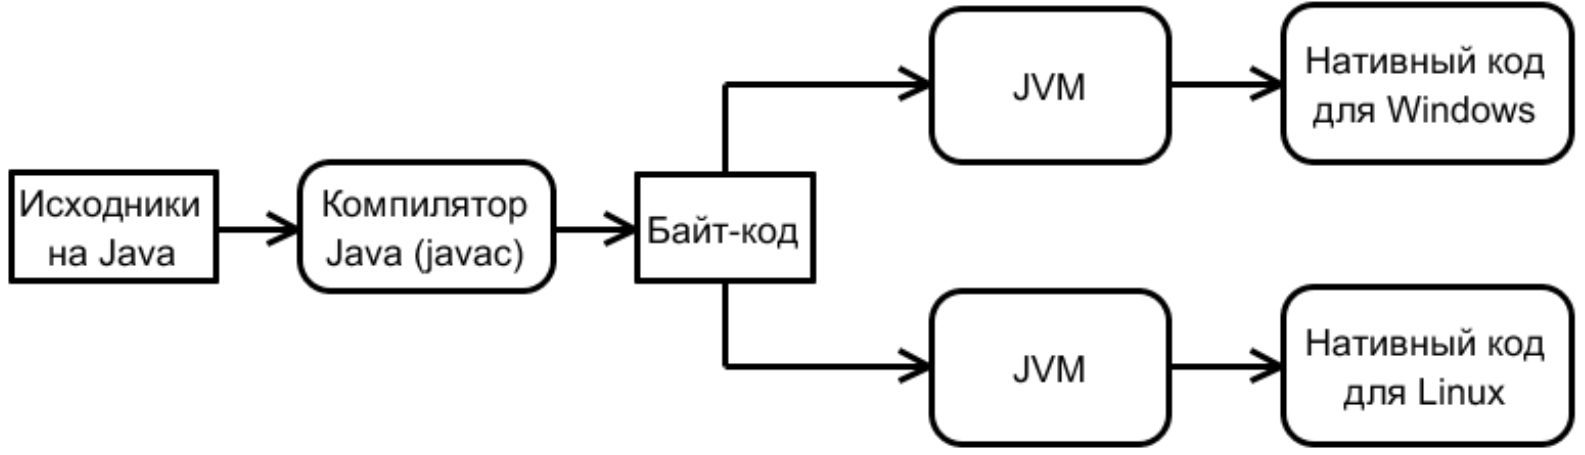
\includegraphics[width=0.8\textwidth]{javaCompiling.png}
	\end{center}
	\caption{Исполнение программы на Java.}
	\label{figure1}
\end{figure}

За такое удобство приходится платить падением скорости работы программы --- ведь интерпретировать инструкцию гораздо дороже, чем просто исполнить её на процессоре. Но существующие Java-машины обычно довольно умные и используют продвинутые техники оптимизации, например Just In Time-компиляцию (это когда последовательность инструкций переводится в машинный код прямо в процессе выполнения программы, а затем запоминается для последующего использования). Многие Java-машины умеют также оптимизировать код на лету, получая данные для оптимизации во время работы программы. Есть и аппаратные реализации Java-машин --- на них Java-приложения могут работать в реальном времени. Вообще, Java-машин очень много, от разных производителей, они предназначены для разных задач --- бывают встроенные в браузеры Java-машины, бывает Java-машина, распространяемая самой Sun вместе со средствами разработки Java, есть Java-машины для мобильных телефонов, карманных компьютеров, и т.д. Следует отметить, что виртуальную машину в качестве среды выполнения использует далеко не только Java --- программы на .NET тоже исполняются .NET-машиной, идея виртуальной машины была предложена ещё Виртом для языка Паскаль. Кстати, важным достоинством виртуальной машины является то, что в её байт-код можно компилировать из сразу нескольких исходных языков, например, в код .NET-машины можно компилировать программы на C\#, C++, Delphi, F\# и т.д., в код Java-машины тоже не одну только Java --- есть ещё языки, типа Скалы, ориентирующиеся на Java-машину как среду выполнения, или Ада --- которая имеет компилятор в байт-код Java помимо нативного кода.

Следующим важным отличием Java от С++ является сборка мусора. В С++ надо было следить за выделением памяти --- память, выделенную в куче, надо было освобождать вручную. В Java выделять память надо, а освобождать --- нет, это сделает сама Java-машина, точнее, сборщик мусора (garbage collector). Java-машина следит за тем, на какие области памяти ссылается программа, и если есть выделенная область памяти, на которую не ссылается больше никто, она её удалит. Опять же, это не особенность Java, .NET поступает так же, а сама идея сборки мусора предлагалась ещё в лиспе, в 1959. Кстати, обратите внимание, что наличие сборщика мусора --- это не повод радостно забить на память и выделять объекты на куче пачками, иначе довольно быстро начнутся проблемы с постоянными вызовами сборщика мусора (а он обычно работает небыстро), фрагментацией памяти и т.д., в общем, за памятью надо следить столь же аккуратно, как и в плюсах, только несколько меньше ручной работы. Плохие новости, кстати, в том, что в Java почти всё выделяется на куче (в C++ программист сам может принимать решение, на стеке или на куче выделять память под тот или иной объект, в Java решение принято раз и навсегда разработчиками языка).

Ещё из концептуальных отличий Java от C++ важны следующие.

\begin{itemize}
	\item В Java (как и во многих остальных современных языках) практически всё является объектом. Например, массивы --- это объекты класса-наследника класса Object (в Java, кстати, все классы наследуют от Object), даже числа, хоть и сами не объекты (они Value Types), приводятся к объектам так называемых обёрточных классов, причём автоматически.
	\item В отличие от C++, где элементарные типы платформозависимы, в Java размер элементарного типа фиксирован спецификацией. То есть, например, int всегда имеет размер 32 бит, long всегда 64 бит (для сравнения, в современном C++ на x86 и x64 int и long --- это одно и то же).
	\item В Java, в отличие от C++, адекватная система модулей, поскольку нет препроцессора и странной системы include-ов. В Java в программе можно использовать имена из любого места кода программы и из любой библиотеки, подключенной к проекту, при этом ничего специально писать не надо. Ну, если использовать полностью квалифицированные имена (вы же знаете, что такое квалифицированные имена и неймспейсы в C++?). Роль неймспейсов в Java играют пакеты (package), отличие в том, что Java довольно фанатично к ним относится --- внутри одного файла может быть только один пакет, причём структура пакетов должна в точности соответствовать структуре папок на диске (отклонение от этого правила --- ошибка компиляции). Например, пакет ru.qreal.kernel должен лежать в папке ru, внутри которой подпапка qreal, внутри которой подпапка kernel. Роль using namespace в Java играет ключевое слово import, роль namespace --- ключевое слово package. Кстати, по стайлгайду пакеты принято именовать, начиная с доменного имени организации-автора пакета, записанного в обратном порядке. Например, если у вас есть домен qreal.ru, то все ваши пакеты лучше именовать ru.qreal.<имя пакета, может быть тоже с подпакетами>. Почему так --- доменные имена глобально уникальны (это обеспечивается службой DNS), так что такая схема именования гарантирует отсутствие конфликтов имён.
	\item Java, как и любой уважающий себя managed-язык (то есть компилирующийся в байт-код), хранит в скомпилированной программе довольно много информации о её статической структуре, которой можно пользоваться во время выполнения. Например, каждый объект имеет ссылку на свой класс, и может спросить, например, своё имя и список своих методов. В C++ ничего такого нет, вся такая информация не переживает компиляции. Это несколько увеличивает требуемый программе объём памяти, но всякие штуки типа плагинов можно реализовать ``прямо из коробки'', да и, например, системы модульного тестирования писать на Java гораздо проще. Библиотека модульного тестирования может сама найти и запустить модульные тесты, практически без помощи программиста. Ещё, кстати, есть такая вещь, как атрибуты, это вообще произвольная информация, которой может быть помечен узел абстрактного синтаксического дерева программы. Они, в совокупности с возможностью генерировать байт-код ``на лету'', позволяют писать полиморфный код и вообще делать всякие ужасные вещи (что активно используется в аспектно-ориентированной парадигме программирования). На C++ такое не сделать.
	\item В Java 8 наконец появились лямбда-функции, функциональный интерфейс для работы с коллекциями (функции типа map, fold, filter и т.д.). В C++ оно тоже появилось, причём на три года раньше, чем в Java, тут надо отдать C++ должное. К тому же, в Java лямбда-функции реализованы довольно неудобно, но лучше так, чем никак.
	\item В Java по историческим причинам, связанным с необходимостью поддержки обратной совместимости, очень странная поддержка шаблонов. Она радикально отличается от C++ (ну, C++ в плане шаблонов вообще особый язык, и ещё неизвестно, хорошо это или плохо). В Java шаблоны называются генериками и они концептуально более честные, чем в C++ (реализуют ``честный'' параметрический полиморфизм, то есть для разных инстанциаций одного шаблона исполняется один и тот же код, в отличие от C++, где каждая инстанциация --- это свой отдельный кусок машинного кода, что делает шаблоны C++ больше похожими на макроподстановку, чем на шаблоны). Проблема генериков в Java в том, что в ранних версиях Java их не было, а сохранить обратную совместимость со старыми Java-машинами (некоторые из которых реализованы аппаратно) было надо, поэтому в байт-коде Java до сих пор понятия ``генерик'' нет. Вот так, шаблон --- структура времени компиляции, во время выполнения программа вообще ничего не знает про шаблоны, что приводит к довольно забавным концептуальным проблемам типа невозможности создать объект параметра-типа.
\end{itemize}

Если что-то из списка выше было непонятно, это абсолютно нормально, про все подобного рода вещи я буду рассказывать дальше, так что можно относиться к этому как к краткому содержанию следующих серий.

\section{Технические детали}

<дальше демострация на проекторе, запускаем IntelliJ IDEA>

Теперь можно перейти к техническим деталям. Создаём новый проект типа ``Java Hello, world application''. Получаем что-то такое:

\begin{minted}{java}
public class Main {
    public static void main(String[] args) {
        System.out.println("Hello World!");
    }
}
\end{minted}

Что мы тут видим: во-первых, работающая программа на Java, как и на любом другом ОО-языке, представляет собой набор объектов, взаимодействующих друг с другом. Тип объекта --- это класс. При этом в Java, в отличие от C++, нет свободных функций, то есть вообще весь код должен быть написан в каком-нибудь классе. Разделения на хедеры и cpp-шники в Java нет, всё, что относится к одному классу, пишется в одном файле, с расширением .java. Считается хорошим тоном поддерживать соответствие "один файл - один класс". При этом каждый класс относится к некоторому пакету, пакеты могут быть вложенными. Если имя пакета не задано, класс относится к пакету по умолчанию, который нельзя импортировать, так что использовать его не рекомендуется, давайте сразу же укажем пакет:
package example;

\begin{minted}{java}
    public class Main {
    public static void main(String[] args) {
        System.out.println("Hello World!");
    }
}
\end{minted}

Пакеты предназначены для организации классов и отвечают за видимость классов друг другу, кроме того, одноимённые классы из разных пакетов можно различить, указывая квалифицированное имя класса: <имя пакета>.<имя класса>. Всё это очень похоже на пространства имён C++. Как я уже говорил, структура вложенности пакетов должна соответствовать структуре вложенности папок в файловой системе, то есть пакету соответствует папка с исходниками. Первой строкой в файле должна быть конструкция package, которая говорит, к какому пакету относится всё, что в этом файле описано. В принципе, package можно не писать, тогда содержимое файла попадёт в пакет по умолчанию, но это невежливо.

Дальше мы видим объявление класса Main. Модификатор доступа public говорит компилятору, что этот класс должен быть виден (то есть, его можно использовать) и в других пакетах. Если этого не написать, класс будет видим только в своём пакете.

Внутри фигурных скобочек находятся объявления полей и методов класса, вложенных классов, перечислений  и т.д. В нашем случае в классе есть только метод main, который во-первых, public --- то есть относится к интерфейсу класса и может быть использован другими классами, которым виден класс Main, во-вторых он static --- то есть он является методом класса, в противоположность обычным методам, которые относятся к конкретному объекту. Всё как в  С++, разве что модификаторы видимости надо писать перед каждым полем и методом. Кроме того, другие соглашения касательно умолчаний, в Java, если модификатор видимости не указан, принимается по умолчанию пакетная видимость. Поэтому модификаторы видимости лучше указывать явно, метод, который мог бы быть private, но из-за отсутствия модификатора доступа имеет пакетную видимость --- нарушение инкапсуляции и может стать причиной незачтённой домашки.

Продолжим смотреть на код. В отличие от С++ "функция" main является методом класса, кроме того, не возвращает код возврата и принимает только массив аргументов (в C++ она вынуждена принимать ещё и количество аргументов, в Java массив сам знает свой размер, как vector в C++, так что main принимает один параметр). Как и в C++,  это список аргументов командной строки, переданных программе, но в отличие от C++ аргументы не содержат исполняемого файла программы, потому что у Java понятие ``исполняемый файл'' весьма растяжимо. При желании эту информацию можно вытащить рефлексией.

Дальше стоит вызов метода println статического объекта out класса System. У out есть ещё много всяких полезных методов, например, метод форматированного вывода, типа сишного printf: System.out.format("\%d", 239);, ну и просто print, который делает то же самое, что и println, но строку не переводит. Заметьте, println может выводить всё без всякой форматной строки.

Синтаксис тел методов весьма похож на C++, так что скорее всего получится просто сесть и начать писать код так, будто бы это был С++. Например, цикл for:

\begin{minted}{java}
for (int i = 0; i < 300; ++i) {
   System.out.println("Hello World!");
}
\end{minted}

Функции делаются, например, так:

\begin{minted}{java}
private static int factorial(int n) {
   if (n == 1)
       return 1;
   return n * factorial(n - 1);
}
\end{minted}

и вызываются так:

\begin{minted}{java}
public static void main(String[] args) {
   System.out.format("Hello, %d", factorial(5));
}
\end{minted}

--- это нужно писать в классе Main на том же уровне, что и функция main. Компилятор многопроходный, поэтому ему плевать, выше или ниже функции main описана наша функция (опять-таки, в отличие от C++).

Про элементарные типы данных вы, я думаю, в состоянии найти информацию самостоятельно, благо они примерно такие же, как в C++ (но помните про стандартизацию размеров), и булевый тип называется boolean, а не bool. Никаких unsigned, long long и прочего в джаве нет, зато в стандартной библиотеке есть класс BigInteger (java.math.BigInteger), который реализует длинную арифметику вообще без ограничений на размер числа.

Есть ещё так называемые оболочечные классы, соответствующие каждому из простых типов, о том, что это такое на самом деле и зачем надо, в следующий раз, пока лишь отмечу полезные статические методы. Например, как преобразовать строку в число:

\begin{minted}{java}
int ololo = Integer.parseInt("239");
\end{minted}

Оболочечные классы (wrapper classes) называются так же, как и примитивные типы, только с большой буквы, и не Int, а Integer, и не Char, а Character.

Массивы: 

\begin{minted}{java}
int[] a = new int[10]; 
\end{minted}

(обратите внимание на странное положение квадратных скобок)

\begin{minted}{java}
for (int i = 0; i < a.length; ++i)
{
   a[i] = i;
}
\end{minted}

Структур в джаве нет, их роль играют классы, что приводит к некоторым проблемам, о которых, видимо, на следующей паре. Пример описания класса:

\begin{minted}{java}
public static class Point {
   public int x;
   public int y;
}
\end{minted}

Есть типы-перечисления:

\begin{minted}{java}
enum Grade {
   EXCELLENT,
   GOOD,
   SATISFACTORY
}
\end{minted}

Они больше похожи на enum class из C++11, в том смысле, что они ``сами себе пространство имён'' (кстати, в Java не надо точки с запятой в конце определения), и использовать их надо примерно так:

\begin{minted}{java}
Grade grade = Grade.EXCELLENT;
if (grade == Grade.SATISFACTORY) {
   System.out.println("Fail");
}
\end{minted}

Константы задаются с помощью ключевого слова final --- если в классе: \mintinline{java}|private final double PI = 3.14;|, если в методе --- без модификатора доступа.

Всякие математические штуки находятся в классе Math. Например, Math.cos(1);

Ещё можно выводить не в консоль, а сразу на графическое окошко. Окошко --- это класс, описанный в пакете javax.swing. Для того, чтобы его можно было использовать, надо сначала импортировать пакет, написав под package, но до public class Main строку import javax.swing.*; --- импортировать все классы из пакета javax.swing (типа С++ного using namespace). Потом в коде программы можно будет написать что-нить вроде

\begin{minted}{java}
JOptionPane.showMessageDialog(null, "Ololo!");
\end{minted}

Можно было сразу написать import javax.swing.JOptionPane; - так мы импортируем конкретно нужный класс, и это считается хорошим тоном. Можно было вообще импорт не писать, а писать в коде javax.swing.JOptionPane.showMessageDialog(null, "Ololo!");  --- по аналогии с C++ным std::string или using namespace std; и затем string;

Так же примерно можно сделать окошко для ввода:

\begin{minted}{java}
String test = javax.swing.JOptionPane.showInputDialog("Ololo!");
\end{minted}

С чтением из консоли дело обстоит несколько хуже: в пакете java.io есть классы BufferedReader и InputStreamReader. Считать строку из консоли можно, например, так:

\begin{minted}{java}
BufferedReader in = new BufferedReader(
    new InputStreamReader(System.in));
try {
   String input = in.readLine();
} catch (Exception e) {
}
\end{minted}

ну или написать в функции main, что она throws Exception. Про исключения в Java потом будет рассказано отдельно, они несколько отличаются от C++-ных исключений, и главное, компилятор Java следит, что все бросаемые методом исключения задекларированы (ну, не все, но про это потом). Ещё, кстати, с какого-то момента так писать будет нельзя, потому что правильнее вот так, но сейчас не время рассказывать, что это значит:

\begin{minted}{java}
try (BufferedReader in = new BufferedReader(
    new InputStreamReader(System.in))) 
{
   String input = in.readLine();
   ...
} catch (Exception e) {
   ...
}
\end{minted}

Что скачать, чтобы всё было --- есть дистрибутив Java SE, лежит на \url{http://www.oracle.com/technetwork/java/javase/downloads/jdk10-downloads-4416644.html}. Бесплатная для студентов и очень годная среда разработки IntelliJ IDEA доступна по ссылке \url{https://www.jetbrains.com/student/}. 

\end{document}
